%!tex root = ../main.tex

%\section{Automatically proving lower bounds for LCL problems} \label{sec:implementation}
\section{Implementation} \label{sec:implementation}
In this chapter we will cover all the important topics that are used in the actual implementation.
The implementation itself is a computer program, that attempts to automatically find a proof which shows the nonsolvability of the given LCL problem in PN model (see section \ref{sec:port_number_model} for more information about PN model).
%TODO should the discussion of the implementation be after explanation of the topics?

\subsection{The idea}
%TODO move the content from this section to 5. Algorithm.
Given an LCL problem, the goal is to find a proof that it is impossible to solve the problem in PN model.
To prove this, we first assume the opposite, that it is possible to solve the problem in PN model.
Then we try to find a counterexample that shows the assumption to be false.
A graph, in which we cannot find any viable labelling, is a good counterexample, as this directly shows that we cannot solve the LCL problem in every graph, therefore it is impossible to solve in PN model.

For each pair of LCL problem and graph, we want to be able to check if labelling is impossible.
To perform the checking, we first encode the problem and graph into a SAT problem.
Then we leverage the power of SAT solvers to solve the SAT problem.
We feed the SAT problem into the solver, which returns either SAT (satisfiable) or UNSAT (unsatisfiable) as a result.
In case the result is UNSAT, we have found a counterexample and we are done.
Otherwise we can continue searching using some other graph.
The routine is illustrated on Figure \ref{fig:implementatio:idea:1}.

\begin{figure}[H]
\centering
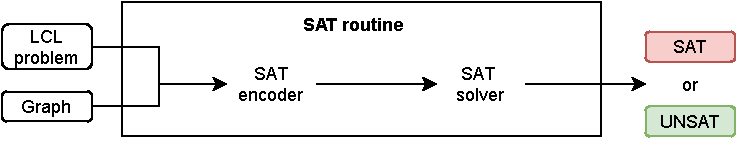
\includegraphics[]{diagrams/implementation_idea_diagram2.pdf}
\caption{The SAT routine. When given a graph and an LCL problem, it checks if a valid labelling exists.}
\label{fig:implementatio:idea:1}
\end{figure}

We repeat the routine for each graph in the current search space and terminate early if the result is UNSAT.
A solid and logical strategy is to first start with the smallest graphs and continue incrementally, increasing the size of graphs  after previous size has been searched entirely.
This can be indeed trivially automated as long as the routine is implemented.
User needs to only input the lower and upper bounds of graph sizes.
Here the graph size is the number of vertices, that is, $n=|V|$.
A search space can be for example every graph from $1$ to $15$.
Then the set of graphs would be $\{(V, E) : |V| \in \{1, 2, ..., 15\} \}$.

\begin{figure}[H]
\centering
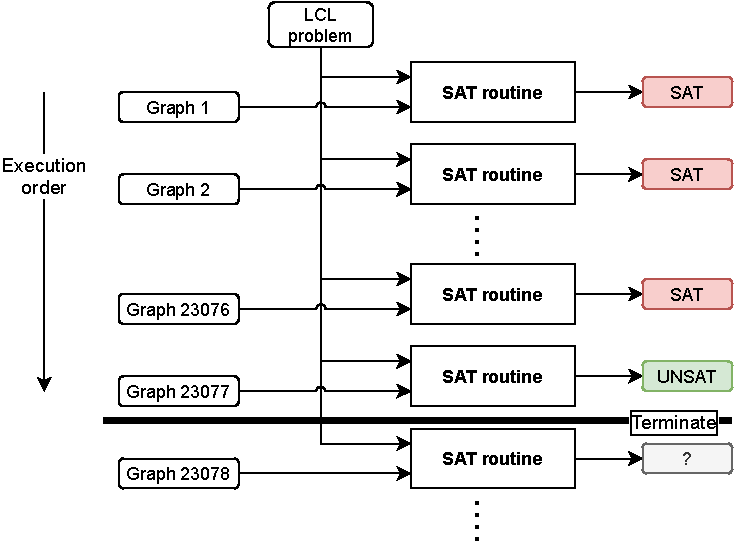
\includegraphics[]{diagrams/implementation_idea_diagram3.pdf}
\caption{An example of an execution of multiple SAT routines. Execution terminates at graph $23077$ when first UNSAT is encountered.}
\label{fig:implementatio:idea:2}
\end{figure}

%TODO biregular multigraphs?
%TODO LCL problems on biregular trees etc?

When we assume that an LCL problem $\Pi$ is solvable in PN, we mean that there exists a deterministic distributed algorithm $A$ in PN model, that finds a solution for all multigraphs i.e. algorithm $A$ works in every multigraph.
Every simple graph is also a multigraph, thus multigraphs are more relaxed in terms of definition.
Allowing parallel edges potentially gives us counter examples with smaller graph sizes when we use the increasing strategy i.e. our algorithm might terminate succesfully much earlier with the desired result and graphs do not necessarily become as complex as they would be with only simple graphs.
%TODO where to discuss about solutions that have been found only with multigraphs? Have we found any solutions with only simple graphs?
Smaller graphs mean less complexity and less performance required but as there are also more graphs to iterate, it is not so simple to justify allowing parallel edges only with this argument.
The main argument is that allowing parallel edges gives us more opportunities to find counterexamples.
It might be that in some problems we cannot even find counterexamples without parallel.

%This is indeed what we have used in this work.
%Probably, we have to iterate a lot of graphs.
%For this purpose we want to be able to generate the graphs.




\subsection{Generating LCL-problems}
%TODO parallelization
\subsection{Generating multigraphs}

%TODO parallelization
\subsection{SAT encoding and solving}
%TODO parallelization?
%\subsection{Software optimizations
\subsection{Caching}
%TODO pre-computing multigraphs and lcl problems and saving them?

\subsection{parallelization}
%TODO Talk about parallelization here or separately in above sections

